A simple two-dimensional nonlinear problem was used to prove the validity of the path-following algorithm.
\begin{mini}
	{x\in\mathbb{R}^2}{p_1x_1^3+x_2^2}{\label{eq:simple}}{}
	\addConstraint{x_2-e^{-x_1}\geq 0}{}
	\addConstraint{x_1\geq p_2}{}
\end{mini}
We start at the approximate solution to Equation \ref{eq:simple}$(x_0,y_0)=((0.5,0.6),1.2)$ with $p=(1,-4)$ and trace a path to generate an approximate solution for $p=(8,1)$.
Note we will refer to $p=(1,-4)$ as $p_0$ or $p_{init}$ and $p=(8,1)$ as $p_f$ or $p_{final}$.
\par
Figure \ref{fig:contour} shows the contour plots and constraints for the approximate solution at $p=(1,-4)$ and at $p=(8,1)$ respectively.
\begin{figure}[H]
	\centering
		\begin{minipage}[b]{0.4\textwidth}
			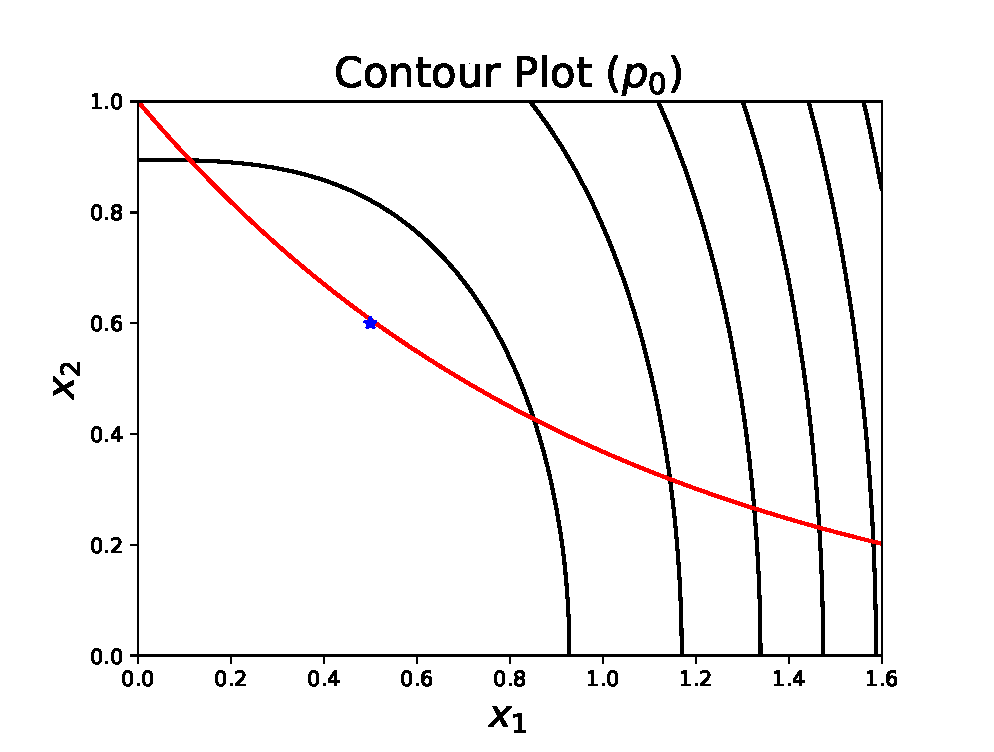
\includegraphics[scale=0.5]{Contour_p0}
		\end{minipage}
		\hfill
		\begin{minipage}[b]{0.4\textwidth}
			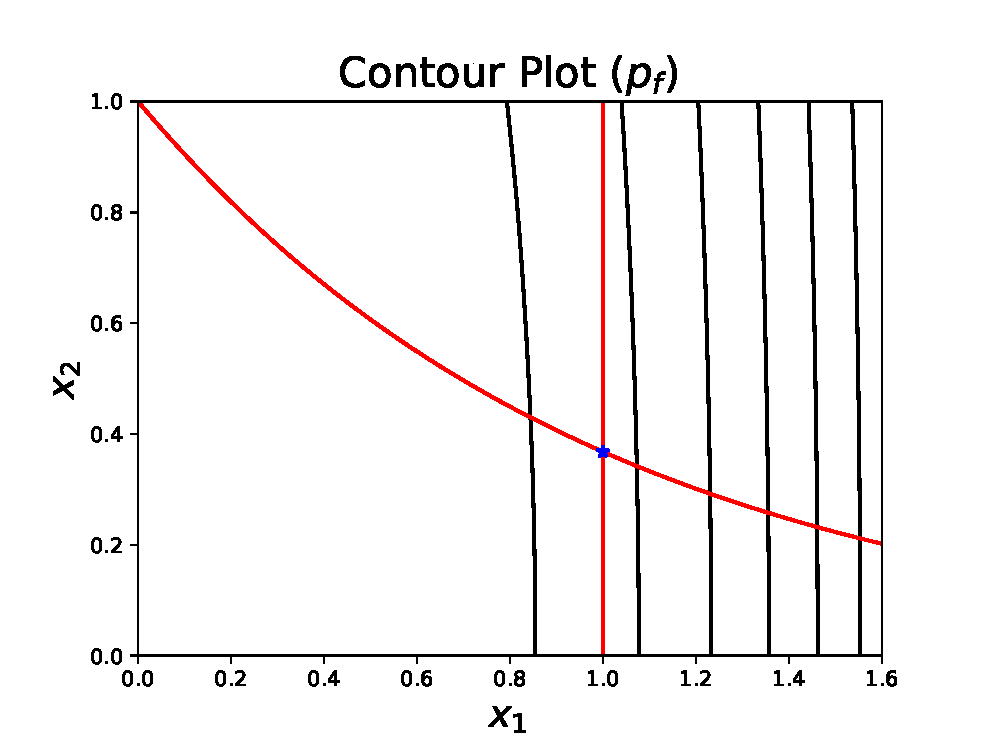
\includegraphics[scale=0.5]{Contour_pf}
		\end{minipage}
	\caption{Plot of the problem at $t=0$ and $t=1$}
	\label{fig:contour}
\end{figure}
The first thing to do before being able to apply any algorithm is to re-write the problem in the more standard NLP form:
\begin{mini}
	{x\in\mathbb{R}^2}{p_1x_1^3+x_2^2}{\label{eq:simple}}{}
	\addConstraint{e^{-x_1}-x_2\leq 0}{}
	\addConstraint{p_2-x_1\leq 0}{}
\end{mini}
We see that this problem has two inequality constraints ($n_{iq}=2$) and zero equality constraints ($n_{eq}=0$).
Algorithm \ref{alg:pathfollowing} is then applied to this problem which requires that the NLP to be solved to find the initial variables: $\boldsymbol{\chi}(\boldsymbol{p}_0),\boldsymbol{\lambda}^*(\boldsymbol{p}_0),\boldsymbol{\mu}^*(\boldsymbol{p}_0)$.
%At $\boldsymbol{p}_0$, the NLP Lagrangian function is given by:
%	\begin{equation*}
%		\Lagrange(\boldsymbol{\chi},\boldsymbol{p}_0,\boldsymbol{\lambda},\boldsymbol{\mu}) = x_1^3+x_2^2+\boldsymbol{\mu}^T\begin{bmatrix}e^{-x_1}-x_2\\-4-x_1\end{bmatrix}
%	\end{equation*}
%Given that there are no equality constraints, $\boldsymbol{\lambda}$ can then be any value and still satisfy the KKT conditions.
%Since we are given that the approximate solution at $p_0$ is $(x_0,y_0)=((0.5,0.6),1.2)$ we can insert this value to find $\boldsymbol{\mu}$.
The NLP solution is then fed to a QP solver where the linearized NLP is solved as a QP.
If the QP is feasible then the primal variables $\boldsymbol{\chi}$ are updated and the dual variables are updated either using the predictor-corrector method.
The step size is then updated as well.
If the QP is infeasible, then we will reduce the step size and try to solve the QP again.
\par
Applying Algorithm \ref{alg:pathfollowing} to this simple problem results in $k$ iterations.
Figure \ref{fig:x1} illustrates $x_1$ with respect to $t$.
The figure shows how $x_1$ changes steeply as the bound constraints become active.
\begin{figure}[H]
	\centering
	\includegraphics[width=\textwidth]{x1}
	\caption{Plot of $x_1$ as a function of $t$}
   \label{fig:x1}
\end{figure}
While this is a simple problem, it is a good test for Algorithm \ref{alg:pathfollowing} since the problem changes substantially both in the nature of the active constraints and the slope of the objective function from $p_0$ to $p_f$\cite{param}.